\chapter{Detail Design}

\section{Relay Switch Circuit}

As explained in section \ref{sec:relay-switch}, a relay switch (the Mantech NT72C 12V DC relay
[\cite{website:relay-specs}]), in conjunction with a 2N2222 Bipolar Junction Transistor (BTJ)
[\cite{website:transistor-datasheet}], is used by the Raspberry Pi to switch the motor on and
off. See Figure \ref{fig:relay-switch} for the circuit diagram.

\begin{figure}[h]
\centering
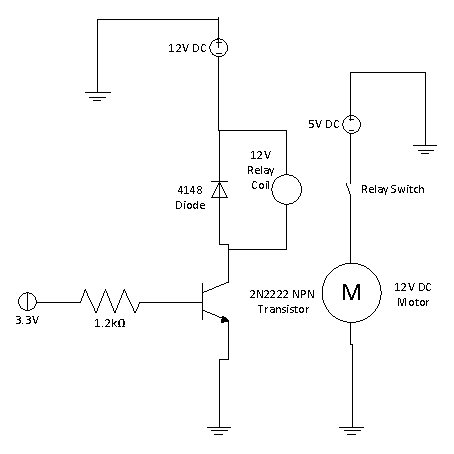
\includegraphics[scale=0.7]{relay_switch.eps}
\caption{12V relay transistor switch. }
\label{fig:relay-switch}
\end{figure}

The relevant  parameters for these components are [\cite{website:relay-specs},
\cite{website:transistor-datasheet}]:

\[ P_{relay} = 0.36W\]
\[ V_{relay} = 12V\]
\[ \beta_{transistor} \approx 10\]
\[ V_{pi} = 3.3V\]

From the relays power dissipation and voltage, its current draw is found by

\[
I_{relay} = \frac{P_{relay}}{V_{relay}}
\]

which gives a current draw of

\[
I_{relay} = 0.03A
\]

Taking the BJT's current amplification as roughly 10, the current draw from the Pi to the
base of the BJT is given by

\[
I_{base} = \frac{I_{relay}}{\beta} = \frac{I_{collector}}{\beta}
\]

This gives a current draw of

\[
I_{base} = 0.003A = 3mA
\]

The maximum current draw from the GPIO pins is 16mA [\cite{website:gpio-specs}], though this is
not recommended as the Pi does not have any current limiting or over-current protection.
Therefore, a current draw of 3 mA is completely safe.

To limit the current draw from the Pi, a base resistor must be added between the Pi's GPIO pin
and the BJT's base. With a current draw of $3mA$ and a voltage of $3.3V$, the resistor size is
found by Ohm's law as follows

\[
R_{base} = \frac{V_{pi}}{I_{pi}}
\]

which gives

\[
R_{base} = 1.1k\Omega
\]

Compensating for tolerances by adding 10\%, the resistor size is set to

\[R_{base} = 1.2k\Omega\]

\section{server program}
\subsection{nfc}
\subsection{qr code}

\section{vending program}
\subsection{nfc}

Because the Arduino version of this shield is locally available, and the cost issues related
to importing a NFC chip that is made for the Raspberry Pi, the Arduino version was bought for 
R780.00. Its Transistor-Transistor Logic (TTL) serial interface was configured in such a way
so that it can serially communicate with the Raspberry Pi's UART interface. It can be powered
by the 5V output pin from the Raspberry Pi. 

\subsection{qr code}

\section{Android app}

\section{Motor and coil}
\label{sec:detail-switch}